\documentclass[12pt,a4paper,oneside]{book}
\usepackage[utf8]{inputenc}
\usepackage[english]{babel}
\usepackage{amsmath}
\usepackage{amsfonts}
\usepackage{amssymb}
\usepackage{makeidx}
\usepackage{graphicx}
\usepackage[left=2cm,right=2cm,top=2cm,bottom=2cm]{geometry}
\author{MehulKumar Sutariya}
\title{{\bf{\Huge ChemDraw}}\\{\large Python Reference}}
\date{}
\begin{document}
\maketitle
\section*{Preface}
Here, most of the problem which is face by me while creating this software are mention! I assume that you know the basic of Python and PyQt.
\chapter{Qt Designer}
\section{LayOut}
There must have to be no any sign of red block in `Object inspector', It create conflicts in the ui.\\
To remove this block ensure that you add geometry for particular Widget(not by manually, you must have to add it by right click on Graphical view of that Widget in Designer); This make sense when you change the size of window after executing.\\
If all requirements by Widget are not full fill then also there is red block symbol.\\
Let's understand this both case by one Figure
\begin{figure}[h]
\centering
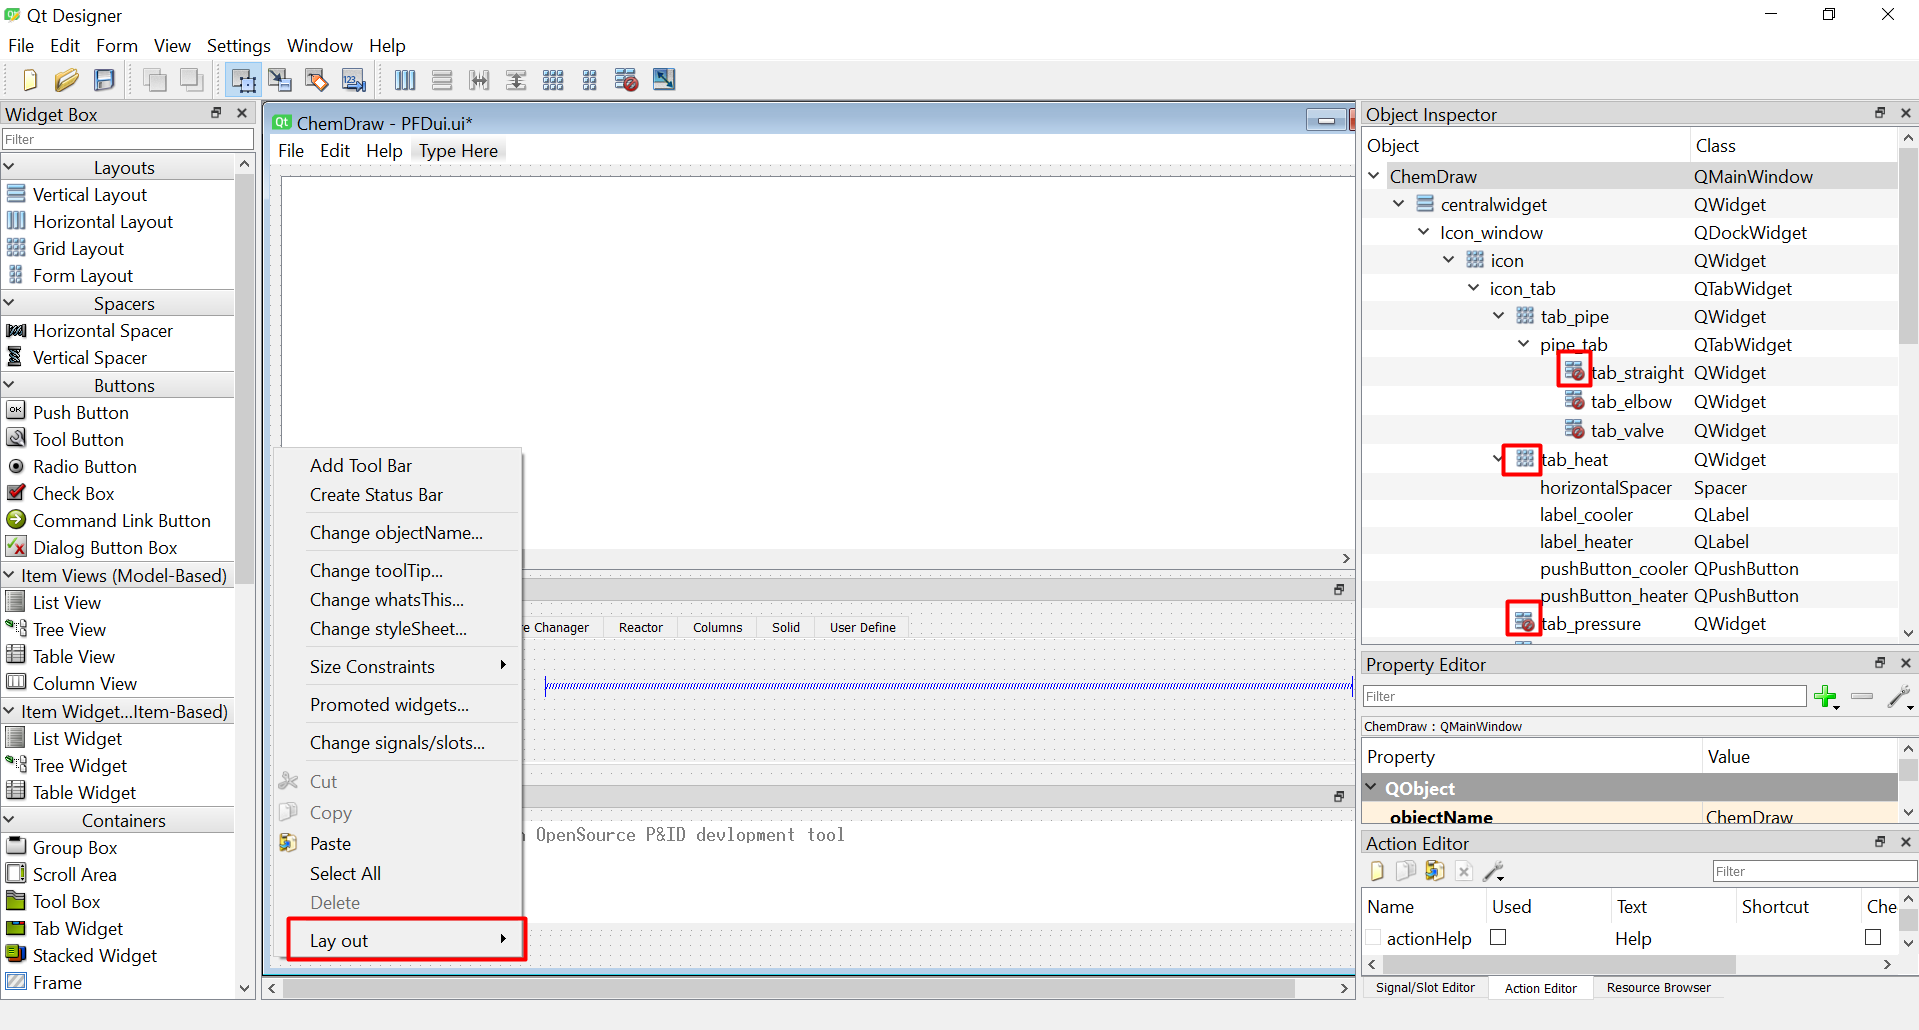
\includegraphics[scale=0.4]{SS/layout.png}
\caption{QtDesigner Window}
\end{figure}
Let's understand this image. Here, you can see some red rectangle;Focus on them. When   right click after adding the appropriate Widget to my `ui' and click right click base dialogue box, outside of any Widget, there is one option called `Layout' after clicking on this you find some option for layout arrangement select appropriate(for ChemDraw it is Vertical), and as soon as you add layout, Red block symbol from ChemDraw(In Object Inspector, at Top Right corner) (QMainWindow) are flew away!\\
See the suboption of pipe\_{tab}, there you find redblock,because there is no any item inside that tab, but see at the heat\_{tab} there is no any block sign because at this moment there is two icon for heater and cooler(Tab view ask minimum one item inside them).\\
Also look at the `Property Editor' window just below the `Object Inspector'; Here, you find some basic but important Option like;
\begin{itemize}
\item ObjectName: You have to give appropriate name to your itme so it is easy to call them when you want to call that item.
\item geometry: It set that item at given position,If your layout is perfectly set then you don't have to bother about it!
\item minimumSize, maximumSize: This both are useful when you don't want you item to be too small or too large then your Expected dimension; They work as their name suggest
\item font: you can set your font style here
\item mouseTracking, tabletTracking: If this are selected only and only then you are able to use mouse event for that Widget
\item WindowTitle, WindowIcon: Must give icon and title if it dialogue box
\item text, icon, iconsize: Select appropriate mode to your item, applicable to text type of item\\
In ChemDraw all icon in icon tab are label!
\item flat: It make transparent background, Don't set opacity to remove the background, it is for whole label not for background.
\end{itemize}
\section{Menubar}
Menubar and status bar can be added directly through the QtDesigner, but you have to focus on the event created by that. There is option of iconic toolbar too!. You can find the event manger or `Action Editor' just below the Property Editor
\chapter{PyQt in Python Code}
Every item and function attached to the parent class are assignable or callable. As example, Think there is QGraphicsView Widget are add in the window; It contain so many child Widget like ScrollBar and function like Mouse Event, Now you can generate new object for that both scrollbar and then this new variable can work as scrollbar but attached with that parent Widget!. Same for `mousemove' and `mousepress' event, you can attach this directly to the appropriate function.
\end{document}